% Please use the skeleton file you have received in the
% invitation-to-submit email, where your data are already
% filled in. Otherwise please make sure you insert your
% data according to the instructions in PoSauthmanual.pdf
%\documentclass{PoS}
%
%\title{Rare and semi-rare decays at ATLAS}
%
%\ShortTitle{Rare decays at ATLAS}
%
%\author{\speaker{Umberto De Sanctis}\thanks{on behalf of the ATLAS Collaboration}\\
%        University of Sussex\\
%        E-mail: \email{umberto.de.sanctis@cern.ch}}
%
%%\author{Another Author\\
%%        Affiliation\\
%%        E-mail: \email{...}}
%
%\abstract{}
%
%\FullConference{16th International Conference on B-Physics at Frontier Machines\\
%		2-6 May 2016\\
%		Marseille, France}
%
%\newcommand{\theInvRho}{\frac{\varepsilon_{\mu^+\mu^-}}{\varepsilon_{J/\psi K^{\pm}}}}
%\newcommand{\pt}{$p_{\rm{T}}$}
%\newcommand{\gev}{\rm{GeV}}
%
%\begin{document}
\section{Measurements of the $B^0_{(s)} \to \mu\mu$ rare decays}
The $B^0_{(s)}$ decays into a pair of oppositely charged muons (referred in the following to as $B^0_{(s)} \to \mu\mu$) is extremely interesting because it is forbidden at lowest perturbative order in the SM due to FCNC suppression and the additional helicity suppression (by a factor of $m^2_{\mu}/m^2_B$). Thus the decay can only proceed through loop diagrams. New heavy particles in extensions of the SM can appear in competing Feynman diagrams and significantly affect the decay branching fractions. Therefore these processes are sensitive to a wide range of new physics phenomena which are not predicted by the SM. Furthermore, thanks to the helicity suppression, the $B^0_{(s)} \to \mu\mu$ branching fractions are accurately predicted in the SM: $BR(B^0_s \to \mu\mu) = (3.65 \pm 0.23) \times 10^{-9}$ and $BR(B^0_d \to \mu\mu) = (1.06 \pm 0.09) \times 10^{-10}$~\cite{Bobeth}. Hence any significant deviations from these predictions would be a hint of New Physics (NP).

Recently, all three Collaborations (ATLAS,  CMS and LHCb) have reported measurements of these branching fractions using full Run I dataset, corresponding to 25 $\rm{fb^{-1}}$ for ATLAS and CMS and 3 $\rm{fb^{-1}}$ for LHCb respectively. CMS and LHCb Collaborations also performed a combined measurement of both branching fractions. The $B^0_s \to \mu\mu$ decay was observed with a $BR(B^0_s) \to \mu\mu) = 2.8^{+0.7}_{-0.8} \times 10^{-9}$ while an evidence of the  $B^0_d \to \mu\mu$ decay, with a  $BR(B^0_d \to \mu\mu) = 3.9^{+1.6}_{-1.4} \times 10^{-10}$~\cite{Nature} was found.
The ATLAS Collaboration has only recently published the measurements, reporting a value for BR($B^0_s) = 0.9^{+1.1}_{-0.8}\times 10^{-9}$ and setting an upper limit at 95\% C.L. on  BR($B^0_d) < 4.2 \times 10^{-10}$.~\cite{ATLAS_Bmumu}

All these analyses extracted both branching fractions simultaneously from a fit in the di-muon invariant mass. In order to minimise the systematic uncertainties affecting the measurement, the branching fractions were evaluated with respect to the same reference channel $B^{\pm} \to J/\psi(\to \mu \mu) K^{\pm}$. Despite the better resolution in invariant mass of CMS and especially of LHCb, ATLAS showed a similar single-event-sensitivity due to a better rejection of the combinatorial and the peaking backgrounds. The latter especially was achieved applying a  multivariate selector based on calorimetric and tracking variables which significantly reduced the contribution of the hadrons (namely $\pi$ and K) that are misidentified as muons. On the other hand, LHCb and CMS provided a better treatment of the partially reconstructed and semileptonic decays contributions in the di-muon invariant mass fit.
In Figure~\ref{fig:BsBd} a summary of the branching fractions measurements performed by the three experiments is shown.

All three experiments consider these measurements crucial in the respective physics programs. All detector improvements described in Section~\ref{intro} will be highly beneficial for all experiments to fully exploit the larger dataset they will collect during the Run II campaign. 
Since these measurements are still statistically limited, ATLAS and CMS can be competitive in Run II with respect to LHCb, given the larger integrated luminosity that the LHC machine will deliver to them. Nevertheless, the capability of the two experiments to keep the di-muon trigger p$_\mathrm{T}$ thresholds as low as possible will be the main challenge in order to maintain the competitiveness in these measurements. The combination of the results of the three experiments using the full Run II expected integrated luminosity will allow to produce a measurement of the $B^0_{(s)} \to \mu \mu$  branching fraction with a precision comparable to the theoretical predictions.
\begin{figure}[!t]
  \begin{center}
    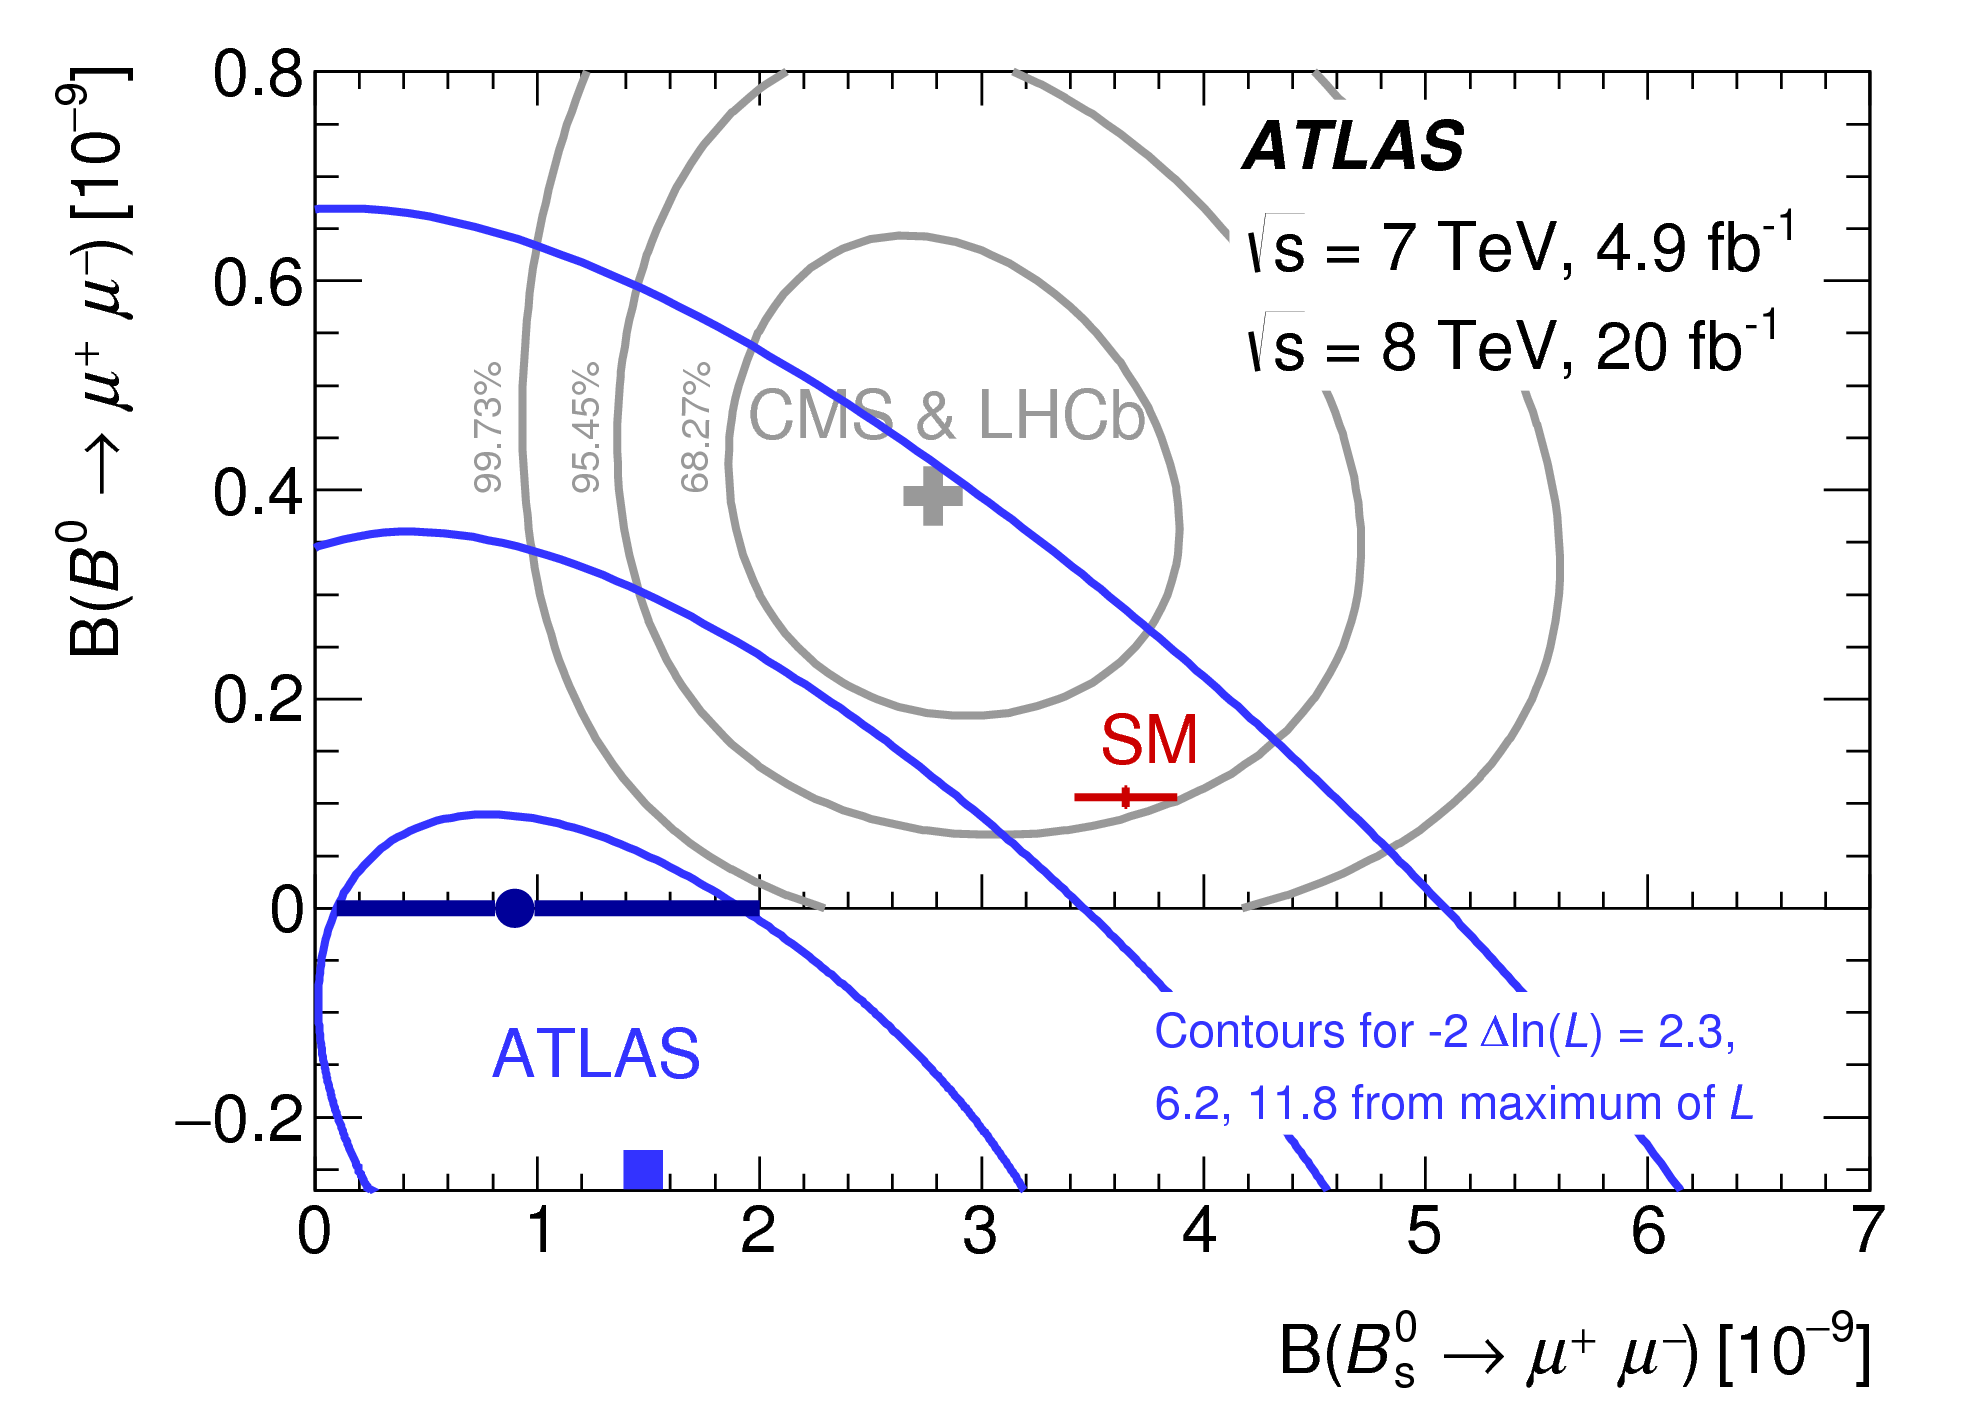
\includegraphics[width=0.6\textwidth]{fig_09.png}
    \caption
        {Contours in the plane  BR($B^0_s \to \mu \mu$), BR($B^0_d \to \mu \mu$) for intervals of
          $-2\, \Delta \ln(L)$ equal to $2.3$, $6.2$ and $11.8$ relative to the absolute maximum 
          of the likelihood (blue square), without imposing the constraint of non-negative branching fractions. 
          Also shown are the corresponding contours for the combined result of the CMS and LHCb 
          experiments, the SM prediction, and the maximum of the likelihood within the boundary of non-negative 
          branching fractions (blue dot), with the error bars covering the 68.3\% confidence range for BR($B^0_s \to \mu \mu$).}
        \label{fig:BsBd}
  \end{center}
\end{figure}

\section{Electroweak penguins decays}
Similarly to $B^0_{(s)} \to \mu \mu$ decays, also $b \to s l^+ l^-$ transitions are suppressed in the SM and thus very sensitive to New Physics processes. These decays are forbidden at the lowest perturbative order and proceed through loops involving electroweak penguin diagrams. Contrary to $B^0_{(s)} \to \mu \mu$ decays, the $b \to s l^+ l^-$ transitions do not have any helicity suppression. This means that possible NP contributions can modify not only the branching ratios of the decays, but also the angular distributions of the particles in the final state. Eventual contributions from NP processes can be parameterised into the SM lagrangian using the effective field theory (EFT) approach. This approach allows to describe any NP contribution simply using higher dimension operators $O_i$ and the energy scale $\Lambda_{NP}$ where NP phenomena should appear. The total lagrangian $L$, which includes NP contributions, can then be written as:
\begin{equation}
L = L_{SM}+\sum_i c_i \frac{O_i}{\Lambda^2_{NP}}
\label{eq:wilson}
\end{equation}
where $L_{SM}$ represents the SM lagrangian and $c_i$ are complex coefficients (called Wilson coefficients) related to the strength of the interaction. In the SM, all $c_i$ coefficients are zero. Any significant discrepancy would then be a hint of the presence of NP phenomena.\\
Several decay topologies involving mesons and baryons that contain $b$-quark belong to this category. One of the most interesting channels is $B^0 \to K^{*0} \mu^+ \mu^-$, where only the $K^{*0} \to K^+ \pi^-$ decay mode is considered. 
The SM predicts a branching ratio of about 4.5 $\times 10^{-7}$, and the full kinematics of the decay can be described by three angles and the invariant mass squared $q^2$ of the two muons in the final state. 
The measurement of the three decay angles and of the differential decay rate as a function of $q^2$ allows to extract specific parameters called $P'_i$ (referred to in the following as optimised observables since they are independent, at the first order, of the form-factors involved in the calculation) which can be directly related to the Wilson coefficients $c_i$ introduced above. \\
The most complete analysis has been performed by LHCb~\cite{mumuK_LHCb}. The branching ratio and the three angles have been measured simultaneously and the full set of $P'_i$ parameters was extracted. A partial angular analysis has also been performed by the CMS Collaboration~\cite{mumuK_CMS}. The analysis led to the extraction of the forward-backward asymmetry $A_{FB}$  measured in the di-muon system. $A_{FB}$ is another observable entering in the formula which describes the differential decay rate for this channel. Both ATLAS and CMS Collaborations are preparing the full angular analysis on the full Run I dataset.  Figure~\ref{fig:mumuK} (left) shows the measurements of the $A_{FB}$ parameter as a function of $q^2$ performed by CMS experiment (compared with the SM prediction~\cite{ABSZ}), while Figure~\ref{fig:mumuK} (right) shows the measurement of one of the optimised observables (namely $P'_5$) as a function of $q^2$,  performed by the LHCb Collaboration (compared with the values obtained by Belle Collaboration~\cite{Belle} and the SM predictions~\cite{DHMV}). A discrepancy of the order of 2.8--3.0 $\sigma$ with respect to the SM predictions, has been reported by LHCb experiment for $q^2$ values between 4 and 8 ${\rm{GeV}}^2$.

Several other decay modes associated with the $b \to s \mu^+ \mu^-$ transition process have been considered by LHCb (such as $B^+ \to K^{+} \mu^+ \mu^-$, $B_s \to  \phi \mu^+ \mu^-$ and $\Lambda_b \to \Lambda \mu^+ \mu^-$). Each of these processes is sensitive to a different set of Wilson coefficients with respect to $B^0 \to  K^{0*} \mu^+ \mu^-$ channel. The differential branching fractions as a function of $q^2$ have been measured for each channel and compared with the SM predictions. Some discrepancy with respect to the SM calculations, even if not significant, has been found also in some of these measurements.
\begin{figure}[!t]
  \begin{center}
  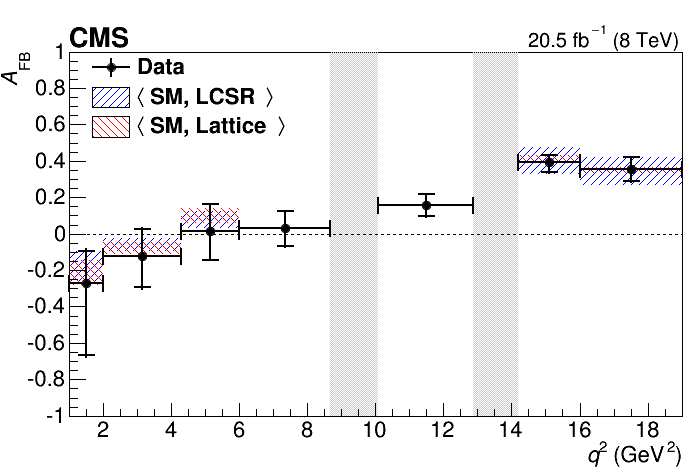
\includegraphics[width=0.48\textwidth]{AFB_CMS.png}
  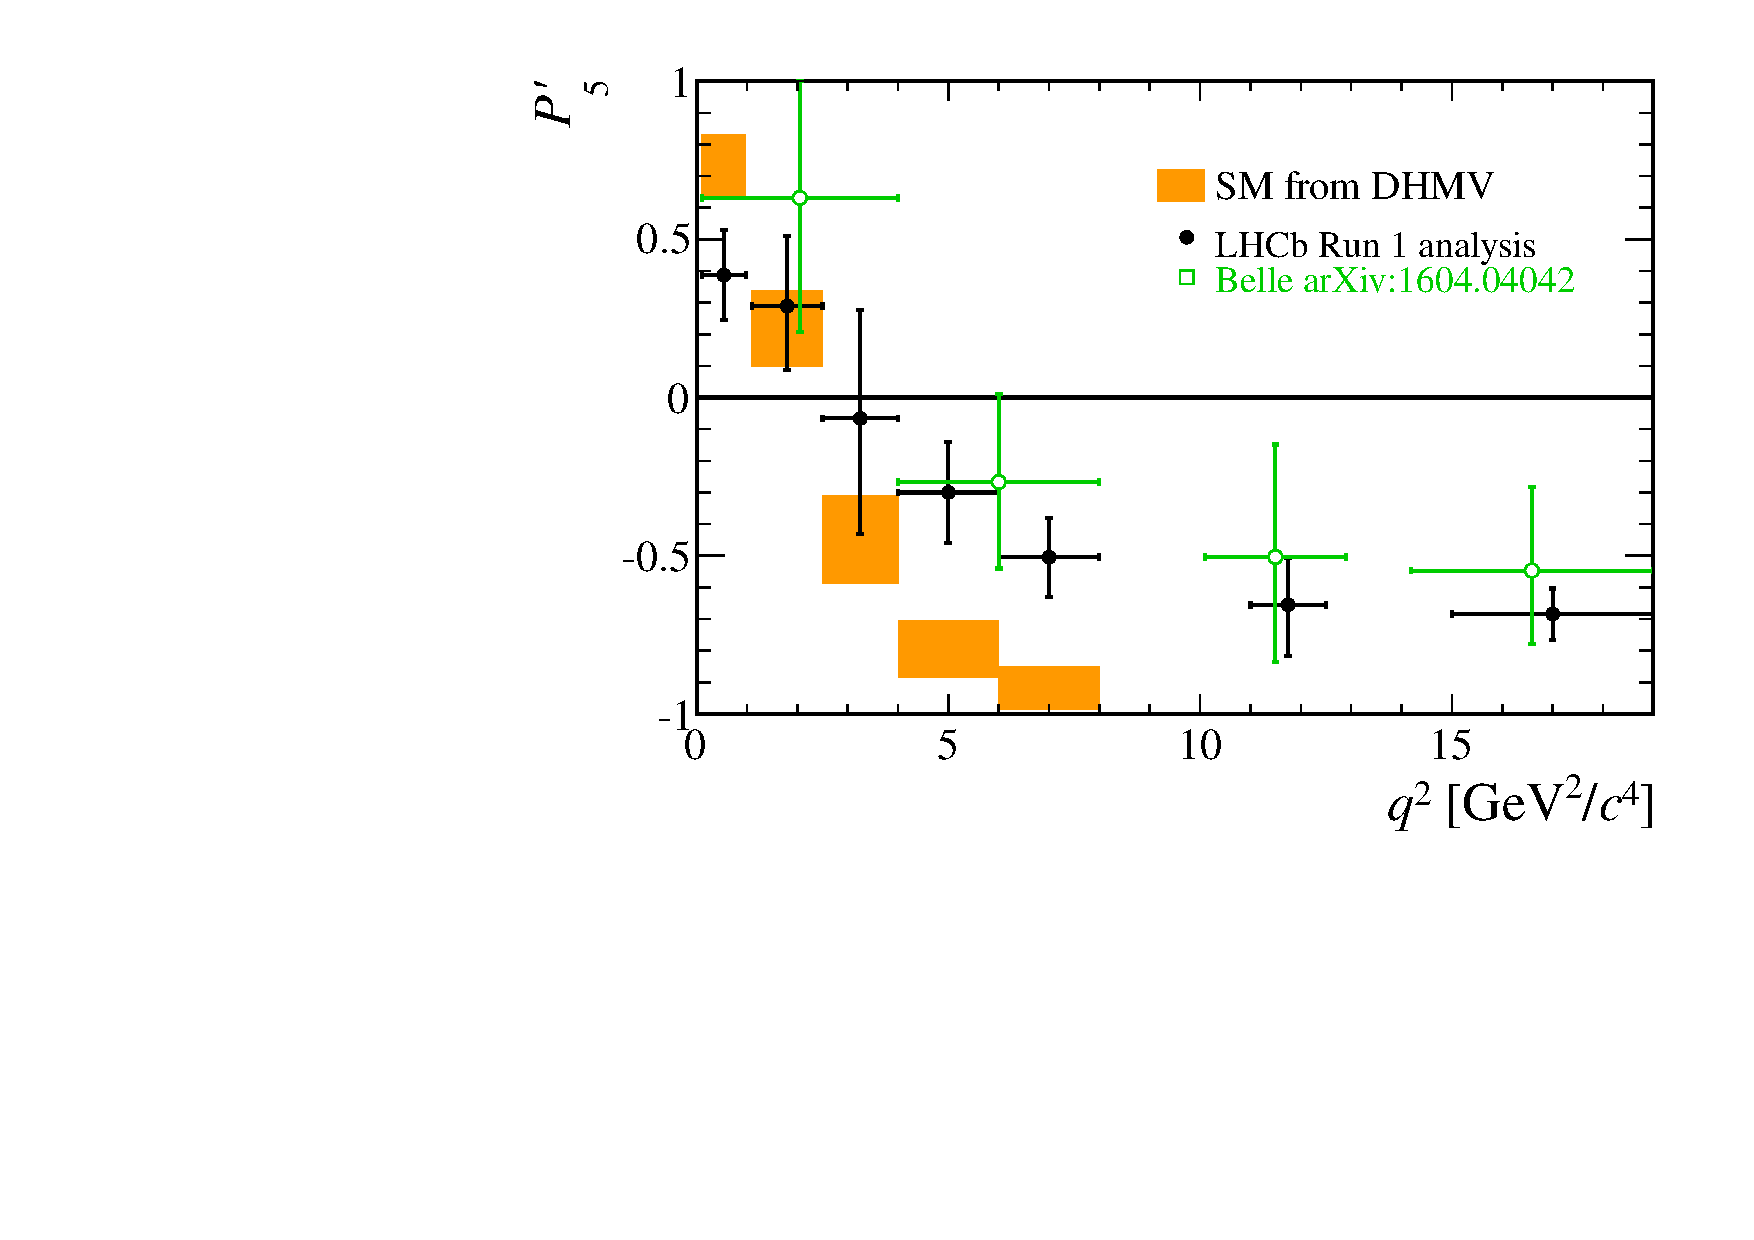
\includegraphics[width=0.48\textwidth]{P5p.pdf}
    \caption {(Left) $A_{FB}$ measurements as a function of $q^2$ as reported from CMS. The SM predictions are taken from~\cite{ABSZ,ABSZ2}. (Right) $P'_5$ distribution as a function of $q^2$ for the measurements performed by LHCb~\cite{mumuK_LHCb}~(black dots) and Belle~\cite{Belle}~(green) Collaborations. The uncertainties include both statistical and systematic components. The SM predictions (yellow bands) are taken from~\cite{DHMV}. }
        \label{fig:mumuK}
  \end{center}
\end{figure}

The plan for the Run II campaign of the three experiments in this domain is to systematically analyse several decay modes related to $b \to s \mu^+ \mu^-$  transitions in order to find any significant discrepancy of the optimised observables with respect to the SM predictions. The LHCb experiment is also planning to perform the same set of measurements using electrons rather than muons in the final state. 
%The use of the electrons in the final state looks instead very complicated for ATLAS and CMS experiments due to the different trigger menus and conditions available for the two experiments.

%\begin{thebibliography}{99}
%\bibitem{Bobeth} Bobeth C. et al., {\it{$B_{s,d} \to l^+ l^-$ in the Standard Model with Reduced Theoretical Uncertainty}}, Phys. Rev. Lett., {\bf{112}}, 101801, 2014.
%\bibitem{Nature} CMS and LHCb Collaborations, {\it{Observation of the rare $B^0_s\rightarrow\mu^+\mu^-$ decay from the combined analysis of CMS and LHCb data}}, Nature, {\bf{522}}, 2015.
%\bibitem{ATLAS} ATLAS Collaboration, {\it{Study of the rare decays of $B^0_s$ and $B^0$  into muon pairs from data collected during the LHC Run 1 with the ATLAS detector}}, arXiv:1604.04263 [hep-ex], 2016. {\it{Submitted to Eur.Phys. J. C}}.
%\bibitem{mumuK_LHCb} LHCb Collaboration, {\it{Angular analysis of the $B^0 \to K^{*0}  \mu^+ \mu^-$ decay using 3~${\rm{fb^{-1}}}$ of integrated luminosity}}, JHEP {\bf{02}} 104, 2016. 
%\bibitem{mumuK_CMS} CMS Collaboration, {\it{Angular analysis of the $B^0 \to K^{*0}  \mu^+ \mu^-$  decay from $pp$ collisions at $\sqrt{s} = 8$ TeV}}. Phys. Lett. B {\bf{753}} 424, 2016.
%\bibitem{Belle} Belle Collaboration, {\it{Angular analysis of $B^0 \to K^{*0}(892) \to l^+ l^-$}}, arXiv:[hep-ex] 1604.04042
%\bibitem{ABSZ} W. Altmannshofer and D.M. Straub, {\it{New physics in $b \to s$ transitions after LHC run 1}}, Eur. Phys. J. C {\bf{75}} (2015) 382 [arXiv:1411.3161].
%\bibitem{DHMV} S. Descotes-Genon, L. Hofer, J. Matias and J. Virto, {\it{On the impact of power corrections in the prediction of $B_d \to K^* \mu^+ \mu^-$ observables}}, JHEP {\bf{12}} (2014) 125 arXiv:1407.8526.
%\end{thebibliography}

%\end{document}
